\chapter{Theoretical Part}

\section{Projectile Shot In An Area Without Air Resistance}

Without the air resistance, the maximum distance that projectile can go, $R$, is calculated as follows:

\begin{equation}
	x_f = x_{\max} = R = v_0 \cdot \cos(\theta) \cdot t
\end{equation}

With this expression in mind, we can find the total flight time as follows:

\begin{equation}
	t = \frac{R}{v_0 \cdot \cos(\theta)}
\end{equation}

And if we use this time to calculate the maximum height, $H$, we can find it as following:

\begin{equation}
	\begin{split}
		H & = y_f = y_0 + v_0 \cdot \sin(\theta) \cdot t - \frac{g}{2} t^2                                                                        \\
		  & = y_0 + v_0 \cdot \sin(\theta) \cdot \frac{R}{v_0 \cdot \cos(\theta)} - \frac{g}{2} \left( \frac{R}{v_0 \cdot \cos(\theta)} \right)^2 \\
		  & = \boxed{y_0 + R \cdot \tan(\theta) - \frac{g}{2} \cdot \frac{R^2}{v_0^2} \cdot \frac{1}{\cos^2(\theta)}}                             \\
	\end{split}
\end{equation}

\section{Finding the General $\tan (\theta)$ Function}

If we leave $\tan (\theta)$ alone in the expression above, we can get a general function for $\tan (\theta)$ as follows:

\begin{equation}
	\begin{split}
		\tan(\theta) R & = H - y_0 + \frac{g}{2} \cdot \frac{R^2}{v_0^2} \cdot \frac{1}{\cos^2(\theta)}                 \\
		\tan(\theta)   & = \boxed{\frac{H - y_0}{R} + \frac{g}{2} \cdot \frac{R}{v_0^2} \cdot \frac{1}{\cos^2(\theta)}} \\
	\end{split}
\end{equation}

\newpage
\thispagestyle{plain}

\section{Developing the $y = f(x)$ Function}

We already have the required function. If we change it a bit, we can develop a general function $y$ as it depends on $x$:

\begin{equation}
	y(x) = y_0 + x \cdot \tan(\theta) - \frac{g}{2} \cdot \frac{x^2}{v_0^2} \cdot \frac{1}{\cos^2(\theta)} \\
\end{equation}

\section{Developing the Envelope Curve}
In order to develop a function, we can manipulate our $y = f(x)$ function a little bit:

\begin{figure}[hbtp]
	\centering
	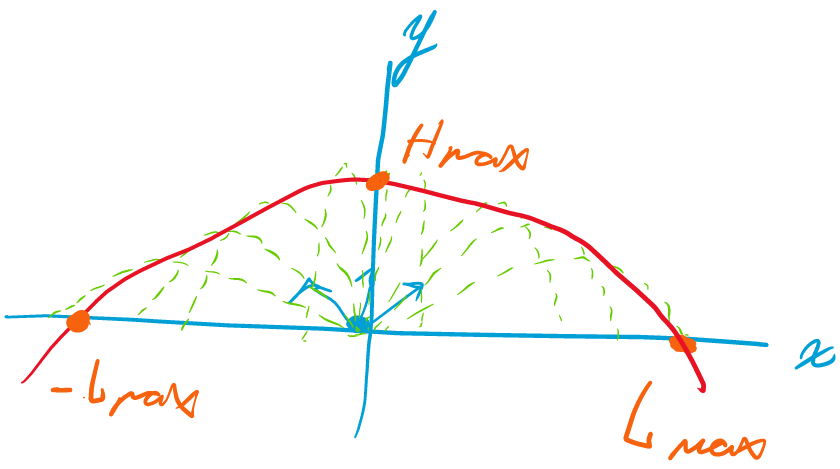
\includegraphics[width=0.8\textwidth]{./assets/envelope.png}
	\caption{Envelope curve of the projectile motion}
	\label{fig:envelope-curve}
\end{figure}

\begin{align*}
	y(x)           & = \tan(\theta)x - \frac{g}{2} \cdot \frac{x^2}{v_0^2} \cdot \frac{1}{\cos^2(\theta)} \\
	\cos^2(\theta) & = \frac{1}{1 + \tan^2(\theta)}                                                       \\
	y(x)           & = \tan\theta x - \frac{g}{2} \cdot \frac{x^2}{v_0^2} \cdot (1 + \tan^2(\theta))      \\
	y(x)           & = \frac{1}{2} \cdot \frac{v_0^2}{g} - \frac{g}{2} \cdot \frac{x^2}{v_0^2}
\end{align*}

\subsection{Finding the Derivative}

\begin{align*}
	\frac{d}{dx} y(x)     & = \frac{-g}{v_0^2} \cdot x \\
	\frac{d^2}{dx^2} y(x) & = \frac{-g}{v_0^2}         \\
\end{align*}
